\chapter{Menghubungkan Lebih Dari 1 Aplikasi Dengan Docker Network}
\section{Pembuka}
Pada panduan kali ini akan membahas mengenai menghubungkan aplikasi menggunakan docker network. Driver docker network yang digunakan adalah bridge.
Kontainer yang dibuat akan dihubungkan dengan docker netwrok agar dapat terhubung.

\section{Langkah menghubungkan lebih dari 1 aplikasi dengan docker network}
\begin{figure}
    1. Cek docker network yang tersedia 

    COMMAND: \textcolor{Blue}{docker network ls}
        \begin{center}
            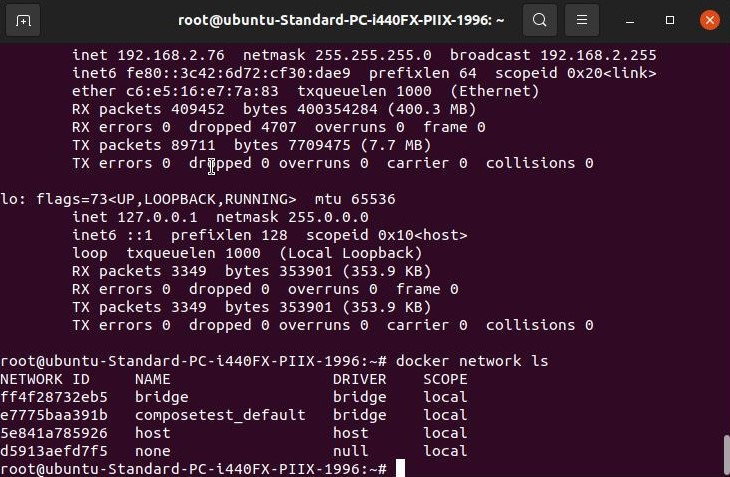
\includegraphics[width=\linewidth]{image/50.jpg}
            \caption{Cek docker network}
            \label{fig:my_figure}
        \end{center}

    2. Buat docker network yang baru menggunakan driver bridge 

    Buat docker network : \textcolor{Gray}{docker network create <DRIVER> <NAMA NETWORK>}

    COMMAND: \textcolor{Blue}{docker network create -d bridge multi-bridge-1}

    lalu cek docker network :

    COMMAND: \textcolor{Blue}{docker network ls}
        \begin{center}
            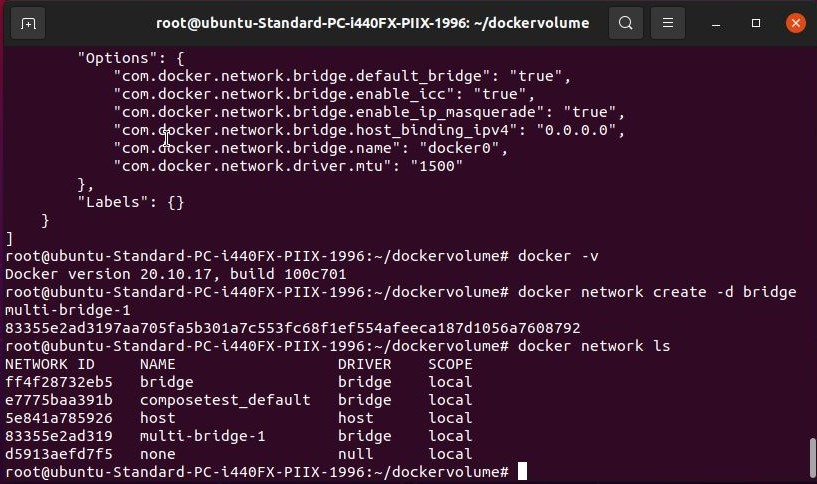
\includegraphics[width=\linewidth]{image/54.jpg}
            \caption{Buat docker network}
            \label{fig:my_figure}
        \end{center}
\end{figure}

\begin{figure}
    3. Buat container baru dan masukan dalam docker network yang sudah dibuat

    Buat container baru dan masukan dalam docker network : \textcolor{Gray}{docker run -itd --network=<NAMA DOCKER NETWORK> <NAMA IMAGE>}
    
    COMMAND: \textcolor{Blue}{docker run -itd --network=multi-bridge-1 rizkiamel23/web:test678}
        \begin{center}
            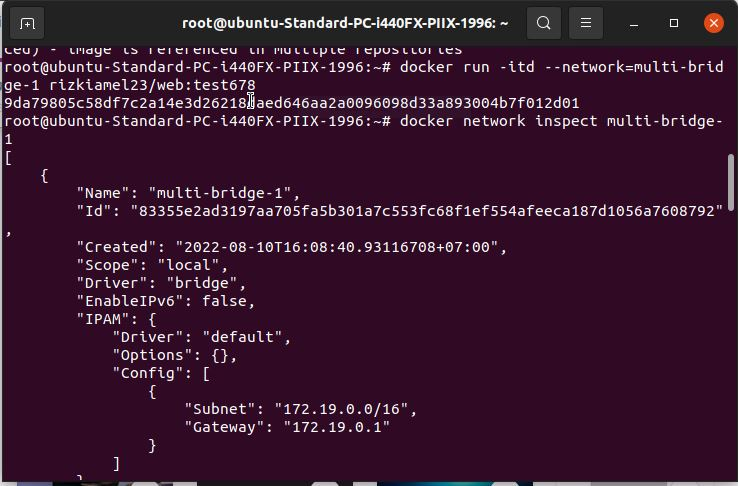
\includegraphics[width=\linewidth]{image/55.jpg}
            \caption{Masukan container ke docker network}
            \label{fig:my_figure}
        \end{center}

    4. Lakukan inspect pada docker network yang sudah dibuat

    Lakukan inspect network : \textcolor{Gray}{docker network inspect <NAMA DOCKER NETWORK>}

    COMMAND: \textcolor{Blue}{docker network inspect multi-bridge-1}
        \begin{center}
            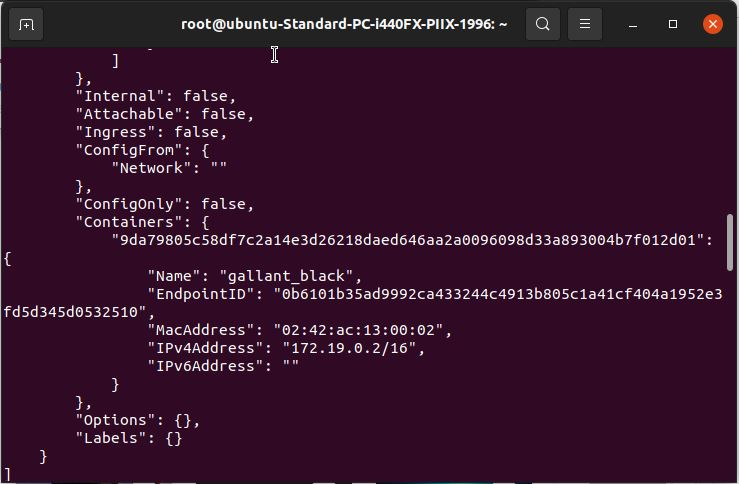
\includegraphics[width=\linewidth]{image/56.jpg}
            \caption{Inspect docker network}
            \label{fig:my_figure}
        \end{center}

\end{figure}

\begin{figure}
    Dari gambar diatas dapat dilihat container yang dibuat tadi masuk ke dalam network docker multi-bridge-1
    
    5.  Jalankan container lainnya

    Jalankan container : \textcolor{Gray}{docker start <ID CONTAINER>}

    COMMAND: \textcolor{Blue}{docker start f99c40dbfacd}
        \begin{center}
            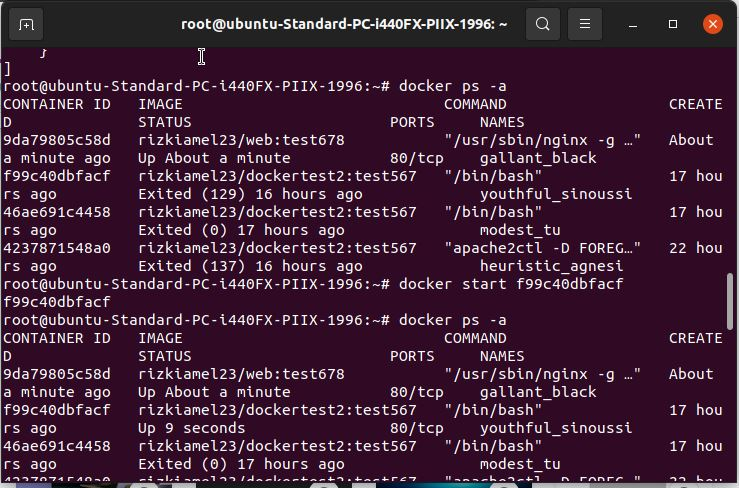
\includegraphics[width=\linewidth]{image/57.jpg}
            \caption{Jalankan kontainer}
            \label{fig:my_figure}
        \end{center}

    6. Tambahkan container ke docker network saat container sedang berjalan

    Tambahkan container ke docker network saat berjalan : \textcolor{Gray}{docker network connect <NAMA DOCKER NETWORK> <ID CONTAINER>}
    
    COMMAND: \textcolor{Blue}{docker network connect multi-bridge-1 f99c40dbfacd}
        \begin{center}
            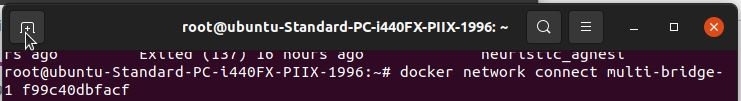
\includegraphics[width=\linewidth]{image/58.jpg}
            \caption{Tambah container ke docker network saat berjalan}
            \label{fig:my_figure}
        \end{center}
\end{figure}

\begin{figure}
    7. Lakukan inspect pada docker network
    
    Lakukan inspect network : \textcolor{Gray}{docker network inspect <NAMA DOCKER NETWORK>}\

    COMMAND: \textcolor{Blue}{docker network inspect multi-bridge-1}
        \begin{center}
            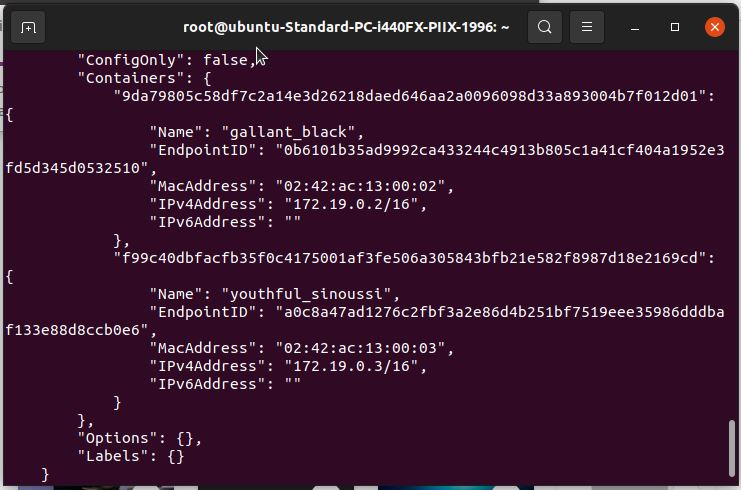
\includegraphics[width=\linewidth]{image/59.jpg}
            \caption{Inspect docker network}
            \label{fig:my_figure}
        \end{center}

    Dari gambar diatas dapat dilihat container yang dijalankan tadi telah ditambahkan pada docker network multi-bridge-1, sehingga kedua aplikasi dapat berkomunikasi dalam jaringan tersebut

    8. Bila ingin memutuskan container dari network 

    Memutuskan container dari network : \textcolor{Gray}{docker network disconnect  <NAMA DOCKER NEWORK> <ID CONTAINER>}

    COMMAND: \textcolor{Blue}{docker network disconnect multi-bridge-1 9da79805c58d}
        \begin{center}
            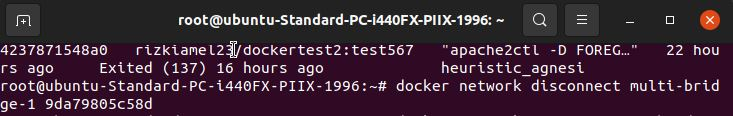
\includegraphics[width=\linewidth]{image/60.jpg}
            \caption{Memutuskan docker network}
            \label{fig:my_figure}
        \end{center}
\end{figure}

\begin{figure}
    Sehingga saat dilakukan inspect multi-bridge-1 list container berkurang
    \begin{center}
        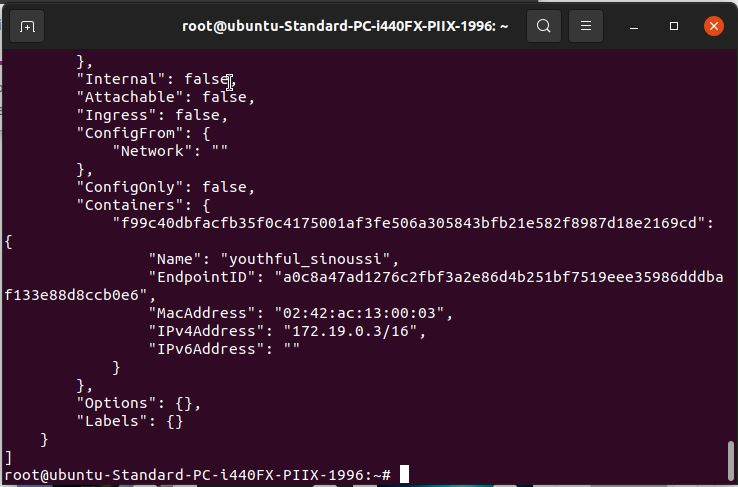
\includegraphics[width=\linewidth]{image/61.jpg}
        \caption{Inspect docker network}
        \label{fig:my_figure}
    \end{center}

    9. Bila ingin menghapus docker network 

    Menghapus docker network : \textcolor{Gray}{docker network rm <NAMA DOCKER NEWORK>}

    COMMAND: \textcolor{Blue}{docker network rm multi-bridge-1}
    \begin{center}
        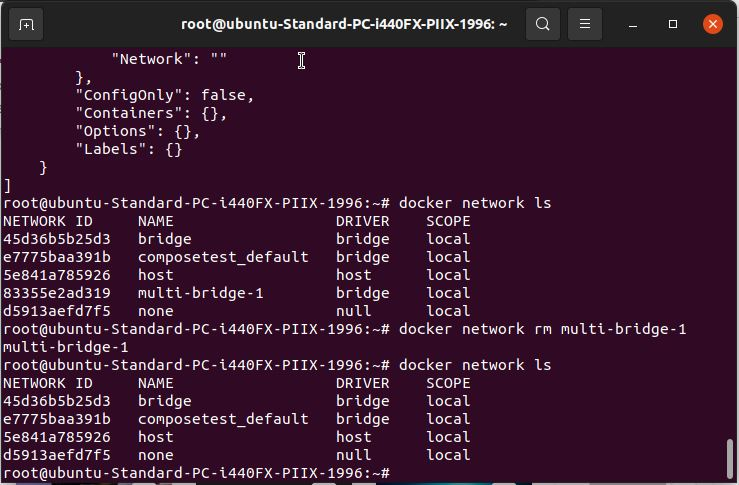
\includegraphics[width=\linewidth]{image/62.jpg}
        \caption{Menghapus docker network}
        \label{fig:my_figure}
    \end{center}
\end{figure}
